\documentclass{article}
%\usepackage[spanish,activeacute]{babel}
%\usepackage[english,activeacute]{babel}
%\usepackage[latin1]{inputenc}
\usepackage[utf8]{inputenc}
\usepackage[english]{babel}

\usepackage{amsmath,amsfonts,amssymb,amstext,amsthm,amscd}
\usepackage{hyperref}
\usepackage{latexsym}
\usepackage{graphicx}
%\usepackage{subfigure}
\usepackage{subfig}
%\linespread{1.6}
\usepackage{float}
\usepackage{dcolumn}% Align table columns on decimal point(esto lo saque del ejemplo de revtex4)
\usepackage{bm}% bold math(esto lo saque del ejemplo de revtex4)
\newcounter{itemR}
\usepackage{here} %recordar usar el comando[H] para las gráficas que es el comando here en lugar de [h!]
\usepackage{fancyhdr}
%\usepackage{sidecap}
%\usepackage[spanish,activeacute]{babel}
\usepackage{multirow}
\usepackage{multicol}
\usepackage{array}
\usepackage{enumitem}
%\usepackage{booktabs}% para hacer tablas profesionales con \toprule

% ------------------------------------------------------------------------------------------------------------------------------------------------------

\usepackage{fancyhdr}
\setlength{\headheight}{15.2pt}
\usepackage[paperwidth=8.5in, paperheight=11.0in, top=1.0in, bottom=1.0in, left=1.0in, right=1.0in]{geometry}

\pagestyle{fancyplain}
\fancyhead[LE,RO]{Práctica $\#$7}
\fancyhead[CE,CO]{}
\fancyhead[RE,LO]{P23-FIS1012-12}
\fancyfoot[LE,RO]{\thepage}
\fancyfoot[CE,CO]{Laboratorio de Física, UDLAP}
\fancyfoot[RE,LO]{}

% ------------------------------------------------------------------------------------------------------------------------------------------------------
% ------------------------------------------------------------------------------------------------------------------------------------------------------
% ------------------------------------------------------------------------------------------------------------------------------------------------------

\begin{document}

\fancypagestyle{plain}{
   	\renewcommand{\headrulewidth}{1pt}
   	\renewcommand{\footrulewidth}{1pt}
}

\renewcommand{\footrulewidth}{1pt}
\renewcommand{\tablename}{Tabla}
\renewcommand{\figurename}{Figura}

% ------------------------------------------------------------------------------------------------------------------------------------------------------
% ------------------------------------------------------------------------------------------------------------------------------------------------------
% ------------------------------------------------------------------------------------------------------------------------------------------------------

\title{Ley de Ohm}
\author{\small{Luis Alberto Gil Bocanegra ID: 177410, Erick Gonzalez Parada ID: 178145}\\
 \small{Gartzen Aldecoa Barroso ID: 178034 .}\\		% ----- Varios autores separarlos por comas:  \small{Nombre(s) de (los) autor(es)\footnote{ID; correo@udlap.mx}, Nombre(s) de (los) autor(es)\footnote{ID; correo@udlap.mx}
	   \small{Depto. de Actuaría, Física y Matemáticas, Universidad de las Américas Puebla, Puebla, M\'exico 72810}}
\date{\small{\today}}

\maketitle

% ------------------------------------------------------------------------------------------------------------------------------------------------------
% ------------------------------------------------------------------------------------------------------------------------------------------------------
% ------------------------------------------------------------------------------------------------------------------------------------------------------

\begin{abstract}
    En esta práctica se identifico la relación de los componentes de la ley de Ohm mediante multímetros 
    conectados a una resistencia que permitió más control midiéndose la resistencia en ohms y la corriente i en ampers, donde nos salieron 
    resultados muy buenos y precisos que avalan la correcta existencia de la ley de Ohm.
\\
\\
{\it Keywords:}  ohms, resistencia 
\\
\\
\end{abstract}

% ------------------------------------------------------------------------------------------------------------------------------------------------------

\begin{multicols}{2}
\section{Desarrollo teórico}\label{Desarrollo Teorico}                              	% -------------------- Introducción
Nuestro objetivo es comprobar la relación entre V, R \& i para un material ohmnico. 
\cite{Fluke}
La Ley de Ohm es uno de los principios fundamentales en la electricidad y la electrónica que describe la relación entre el voltaje (V),
 la corriente (I), y la resistencia (R) en un circuito eléctrico. Fue formulada por el físico alemán Georg Simon Ohm y se expresa matemáticamente de la siguiente manera:

 \begin{equation}
    V = I * R 
 \end{equation}

 Donde:
\\
V representa el voltaje en voltios (V). El voltaje es la fuerza impulsora que impulsa la corriente a través de un circuito. Se mide en voltios y se refiere a la diferencia de potencial eléctrico entre dos puntos en un circuito.
I es la corriente en amperios (A). La corriente eléctrica es el flujo de carga eléctrica a través de un conductor y se mide en amperios. Indica la cantidad de electrones que fluyen por unidad de tiempo.
R es la resistencia en ohmios ($\Omega$). La resistencia representa la oposición al flujo de corriente en un circuito. Cuanto mayor sea la resistencia, menor será la corriente para un voltaje dado. Se mide en ohmios y depende de las características del material y la geometría del componente.
La Ley de Ohm es especialmente útil para calcular voltajes, corrientes y resistencias en circuitos simples. También se utiliza para diseñar y analizar circuitos eléctricos, determinar el valor de las resistencias necesarias y comprender cómo funcionan los componentes electrónicos en un circuito.
En resumen, la Ley de Ohm establece que el voltaje en un circuito es directamente proporcional a la corriente y la resistencia. Es una herramienta fundamental en la teoría eléctrica y se aplica en una amplia variedad de aplicaciones, desde circuitos eléctricos básicos hasta dispositivos electrónicos más complejos.
\section{Desarrollo Experimental}\label{Desarrollo experimental}				% -------------------- Metodología 
\subsection*{Lista de Materiales}
A continuación se presenta una lista de materiales:
\begin{enumerate}
    \item Reóstato 100 Ohms 
    \item Multímetro
    \item Cables banana(2)
    \item Fuente de bajo voltaje 0-24 V
\end{enumerate}
Primero un valor de R, conectamos la fuente y el multímetro para registrar el voltaje
seguido conectamos el multímetro para registrar la corriente, después vamos incrementando el voltaje 
de 1 por 1 y registramos la corriente i, repetimos hasta por lo menos 3 valores distinto de R y por ultimo graficados.  
 \end{multicols}
\section{Resultados y análisis}\label{Resultados}			% -------------------- Resultados

\begin{figure}[H]
    \centering
    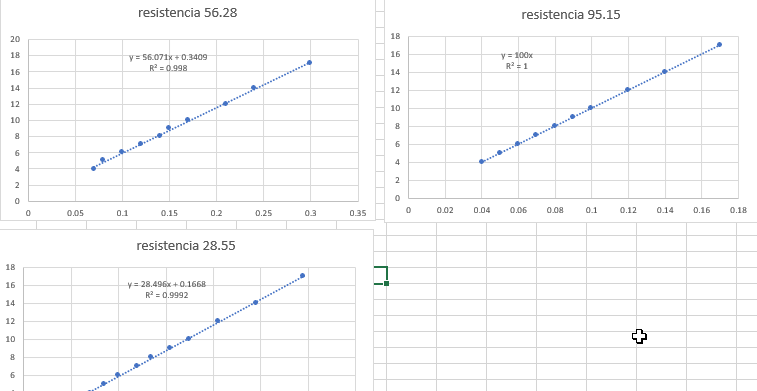
\includegraphics[scale=0.7]{../imgs/r0.png}
    \caption{gráficas individuales}
    \label{fig:1}
\end{figure}

Se puede observar de la fig \ref{fig:1}
que la pendiente corresponde a la resistencia apuntada que deseabamos calcular y el margen
de error fue prácticamente nulo de acuerdo a las gráficas de la figura.
En la gráfica de resistencia 95.28, la función resultó ser completamente lineal debido a que la resistencia era casi de 100 y los valores de voltaje que se iban agregando iban ascendiendo de manera secuencial, osea de 1 en 1. La diferencia con las otras gráficas es que aquellas tenían resistencias de valores menos exactos, por lo que la variación en la gráfica se aprecia por dicho valor.
\begin{figure}[H]
    \centering
    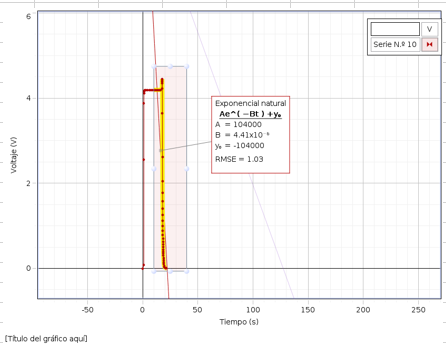
\includegraphics[scale=0.6]{../imgs/r1.png}
    \caption{gráficas juntas}
    \label{fig:2}
\end{figure}

\section{Conclusiones}\label{Conclusiones}				% -------------------- Conclusiones
Como equipo concluimos que el objetivo si cumplió en esta ocasión con básicamente cero error  
Una conclusión importante de la Ley de Ohm con respecto a la resistencia es que, si se mantiene constante la tensión aplicada a un conductor, la corriente que fluye a través de él disminuirá a medida que aumente su resistencia. Por otro lado, si se mantiene constante la resistencia, la corriente aumentará en proporción directa a la tensión aplicada. Esta relación lineal es fundamental para comprender y calcular el comportamiento de los circuitos eléctricos y es ampliamente utilizada en electrónica y electricidad.
\begin{thebibliography}{9}						% -------------------- Bibliografía
	\bibitem{Fluke}
	Fluke. (s. f.). ¿Qué es la ley de Ohm? Fluke. https://www.fluke.com/es-mx/informacion/blog/electrica/que-es-la-ley-de-ohm
	\bibitem{Serway}
	Serway, R. A., $\&$ Jewett, J. W. (2008). Física para ciencias e ingeniería. (7.a
ed., Vol. 1). CENGAGE Learning.

\bibitem{Pérez}
	Newton, I. (1687). Philosophiæ Naturalis Principia Mathematica [Mathematical Principles of Natural Philosophy]. Londini: Jussu Societatis Regiæ ac Typis Josephi Streater.

\end{thebibliography}
\end{document}	